% \documentclass[rnd]{mas_proposal}
\documentclass[thesis]{mas_proposal}

\usepackage[utf8]{inputenc}
\usepackage{amsmath}
\usepackage{amsfonts}
\usepackage{amssymb}
\usepackage{graphicx}

\title{Real-time Learning from Demonstration under Graph-World representation}
\author{Natalia Leonila Quiroga Perez}
\supervisors{Prof. Dr. Paul G. Plöger\\
	Dr. Alex Mitrevski \\}
\date{July 2023}

% \thirdpartylogo{path/to/your/image}

\begin{document}

\maketitle

\pagestyle{plain}

\section{Introduction}

\subsection{Topic of This  Project / Learning from Demonstration }
\begin{itemize}
    \item Provide reasonably detailed description of what you intent to do in your Master Thesis.
    \item You may also discuss the challenges that you have to address.
    \item Reflect on the profile of the reader and PLEAAAASE, tell a story here and refrain from bombarding the readers with details which they may not be able to appreciate.

    Due to the growing acceptance of the use of robots in collaboration with humans in the same environment, Human-Robot Interaction (HRI) is being studied as a successfully emerging area. According to \cite{sheridan2016}, there are four areas of application of HRI; namely, (i) human resources as supervisors in different areas where the tasks are repetitive but robots are still not independent (ii) Robots that work in hazardous environments where humans do not have access, and whose movements are usually controlled remotely by an expert, (iii) autonomous robots, such as self-driven cars with humans as passengers, that navigate and plan by sensing their environment, and finally, (iv) robots in a social environment where they interact directly with people, teaching, entertaining, helping children and the elderly.
    
    Specifically, focusing on human-robot social interaction applications, robots used in therapy with children with Autism Spectrum Disorder (ASD) had a positive impact on the patients, as the children had certain preferences for the robot as a therapist instead of an adult; according to  According to \cite{prabha2019}, this is because children with this condition perceive the world differently and robots attract their attention.
    
    In order to encourage patients with autism to learn movements and body language during therapy, the typical procedure is human-human encounters; namely a selection of imitation games are performed as described in \cite{dautenhahn2004}, they are aware that robots have limited movements and as a long term goal it is difficult to work with them unless the robots increase their behavioural repertoire.
    
    
    Recently, the number of robotics applications in different areas is growing. There are new robots not only in the industrial area, but for everyday applications as well. In the area of health, personal assistance, care and also education, it is intended to include robots in educational, therapeutic and rehabilitation processes \cite{Stein2005}. In the educational context, as part of Human Robot Interaction (HRI), the robot is defined as a social interactor that is in constant contact with human users or agents. This social interaction is intended to be "intelligent", meaning that the robot must interact in a realistic way by giving logical, coherent responses or appropriate gestures. Educational and interactive robots have been developed and marketed since the 1980's and are very popular with young children since then \cite{Sheridan2016}. 
   	
   	
    
    Consequently, different robots have been implemented to interact with children from a very early age as kindergarten assistants \cite{Oliveira2016}, home educational \cite{Jeonghye2005}, and therapy assistance \cite{Vulpe2021}. Many activities can be done by robots during the learning process of children; robots can be especially helpful since teachers see the convenience to develop problem-solving, creativity, critical thinking, and team working, among others \cite{Vostinar2019}. More deeply into the branches of education and health, therapists and teachers of children with Autism Spectrum Disorder (ASD) reported that they are more attracted by toys with dynamic parts like wheels, movable attachments, lights and sounds than by in-animated objects \cite{Qidwai2013}. Robots, due to their characteristics such as predictability in their actions, simplicity of interaction, and repeatability of known states, can be less intimidating and easier to interact than humans. For these particular reasons, they can be especially useful for teaching emotional skills to children with ASD \cite{costa2017socially} and consequently, adapt these mechanisms to regular therapy to enhance learning and integration of patients into society.
    
    Robots are a therapeutic tool for children with autism. Such robots can be classified into three groups: the robot as a therapeutic playmate, the robot as a mediator, and the robot as a model of a social agent \cite{Dautenhahn_2003}. During a therapy, the patient-robot interaction should flow with human-like movements; such actions are part of Social Robotics (SR) conditions and are based on imitation. Aiming at the development of social interactions with robots \cite{Pennazio_2017}, the selected sets of activities chosen by the therapists include imitation games, conversational exchange, and physical interaction. During the last activity, it is common to require repetitive actions from the robot and especially a synergy where the robot performs movements; for instance, the child must replicate the actions to learn about body control and interaction with the environment. Unfortunately, the number of robot movements is often limited, due to the complexity involved in creating new sequences and the requirement of prior knowledge to manipulate the robot. Controlling the posture of robots is especially a difficult task when it is done manually; in particular as the number of robots' Degrees of Freedom (DOF) increases, so does the difference compared to a human's DOF \cite{Fadli2018}. 
    
    The problem identified during this study is the deficiency in the learning process in humanoid robots of new movements coming from human demonstrators or the lack of a complete system that can perform this learning in an efficient, fast and friendly way for the end-user, in this case the therapist. Without neglecting that there are many important considerations to create a friendly learning systems, it is important to consider the following three questions when intending to use imitation learning as a solution for the above mentioned problem: (i) what to imitate or which is the guiding agent, (ii) how to imitate or what are the tools that allow the desired movement, and (iii) when to perform the imitation to avoid unwanted movements \cite{Billard_2004}; these questions help us define the conditions under which the system can be manipulated. According to \cite{lopes2005developmental}, learning by imitation has three main difficulties: how to collect relevant information to perform a task; how to convert data that is valid for a human into a different body, in this case a robot; and how to select the important parts of the demonstration. These points are developed throughout this work and are explained in detail in the following sections.
    
    Learning through imitation consists of observing an agent perform an activity and being able to imitate it as accurately as possible. Using Imitation Learning (IL), the system would be able to learn how to perform similar moves or tasks by observing human performance, avoiding the need for supervised learning or trial and error \cite{lopes2005developmental}. If these long procedures are avoided, then the need for constant technical support to the therapist can be avoided, the process is simplified and ideally proceeds as follows; the needed actions during therapy must be learned; for this, a human guide or operator who decides when a movement starts and ends shows a demonstration to the robot. The creation and configuration of each new movement should take as much time as the user wishes to demonstrate, but not too much additional time to train an algorithm for recognising and reproducing them. This procedure does not require prior knowledge of programming on the side of the therapist, given that the movements will be saved automatically at the end of every demonstration and could be reproduced later for verification, but can also be used during therapy as often as desired.
    
    This research and development project report presents the process of learning through imitation for robots. To this end, we used QTrobot from LuxAI \cite{qtrobot_safety_manual} and considered both its physical and software features. For the overall learning by imitation process, the first step is identified to be the human action recognition, which can be done through the utilization different methods. For this study, we use depth skeleton motions \cite{Chen_2016}, where the teacher's position is calculated with respect to the camera coordinate system placed on the head of the robot; then, the joint angles describing the full-body are found with the use of an analytic solution to reach the desired positions, and, subsequently, Direct Kinematics (DK) with those angles is performed to calculate the end-effector position \cite{Riley}. Secondly, to remove the effect of frames that contain what we call $noise$, we use filters in order to smooth the joint trajectory signal and we also predict possible collisions by the end-effector in order to avoid damage to the robot and all its parts, which is done by means of the re-estimation of angular positions with Inverse Kinematics (IK). Finally, a control system is proposed in order to improve the precision of the robot's movements.
    
    The content of this work report is organized as follows. Chapter 2 provides the background knowledge required for understanding the field of learning through imitation and provides an overview of the state of the art work existing to date, namely the work in the fields of skeleton recognition, forward and inverse kinematics, collision avoidance and control systems. Chapter 3 describes the problem addressed, and the task of this work as a detailed description of the proposed solution. The performance evaluation of the algorithms given in this approach is presented in chapter 4, as a discussion of the results. Finally, the conclusion of this work and aims of the future research are presented in chapter 5.
    
\end{itemize}

\subsection{Relevance of This Master Thesis}
\begin{itemize}
    \item Who will benefit from the results of this project?
    \item What are the benefits? Quantify the benefits with concrete numbers.
    \item 
    \item 
    \item 
 \end{itemize}

\section{Related Work}

\subsection{Survey of Related Work}
\begin{itemize}
    \item What have other people done to solve the problem?
    \item You should reference and briefly discuss at least the ``top twelve'' related works
\end{itemize}

\subsection{Limitation and Deficits in the State of the Art}
\begin{itemize}
    \item List the deficits that you have discovered in the related work and explain them such that a person who is not deep into the technical details can still understand them.
    For each deficit, provide at least two references
    \item You should reference and briefly discuss at least the ``top twelve'' related works
\end{itemize}

\section{Problem Statement}
\begin{itemize}
    \item Which of the deficits are you going to solve?
    \item What is your intended approach?
    \item How will you compare you approach with existing approaches?
\end{itemize}

\section{Project Plan}

\subsection{Work Packages}
\emph{Planning is the replacement of randomness by error.} (Einstein). Very much like you would never start a longer journey without a detailed travel plan, you should not start a project without a carefully though out work plan. A work package is a logical decomposition of a larger piece of work into smaller parts following a ``divide and conquer" strategy. It is very specific to the problem that you are going to address. Refrain from a rather generic decomposition. If your work plan looks similar to those of your school mates, which may address completely different problems then you have not thought carefully enough about how you approach the problem. It is ok to have two generic work packages \emph{Literature Study} and \emph{Project Report}. Discuss your work packages in the ASW seminar.

The bare minimum will include the following packages:
\begin{enumerate}
    \item[WP1] Literature Study
    \item[WP2] ...
    \item[WP3] ...
    \item  ...
    \item[WPy] Evaluation of approach and comparison with similar approaches
    \item[WPz] Project Report
\end{enumerate}

\subsection{Milestones}
Milestones mark the completion of a certain activity or at least a major achievement in an activity. Milestones are also decision points, where you reflect on what you have achieved and what options you have for continuing your work in case you have not achieved what was planned. Above all, milestones have to be measurable. As above, if your milestones are the same as those of your school mates, then you may not have thought carefully enough about how your project shall progress.
\begin{enumerate}
    \item[M1] Literature review completed and best practice identified
    \item[M2] ...
    \item[M3] ...
    \item[M4] Report submission
\end{enumerate}

\subsection{Project Schedule}
Include a Gantt chart here. It doesn't have to be detailed, but it should include the milestones you mentioned above.
Make sure to include the writing of your report throughout the whole project, not just at the end.

\begin{figure}[h!]
    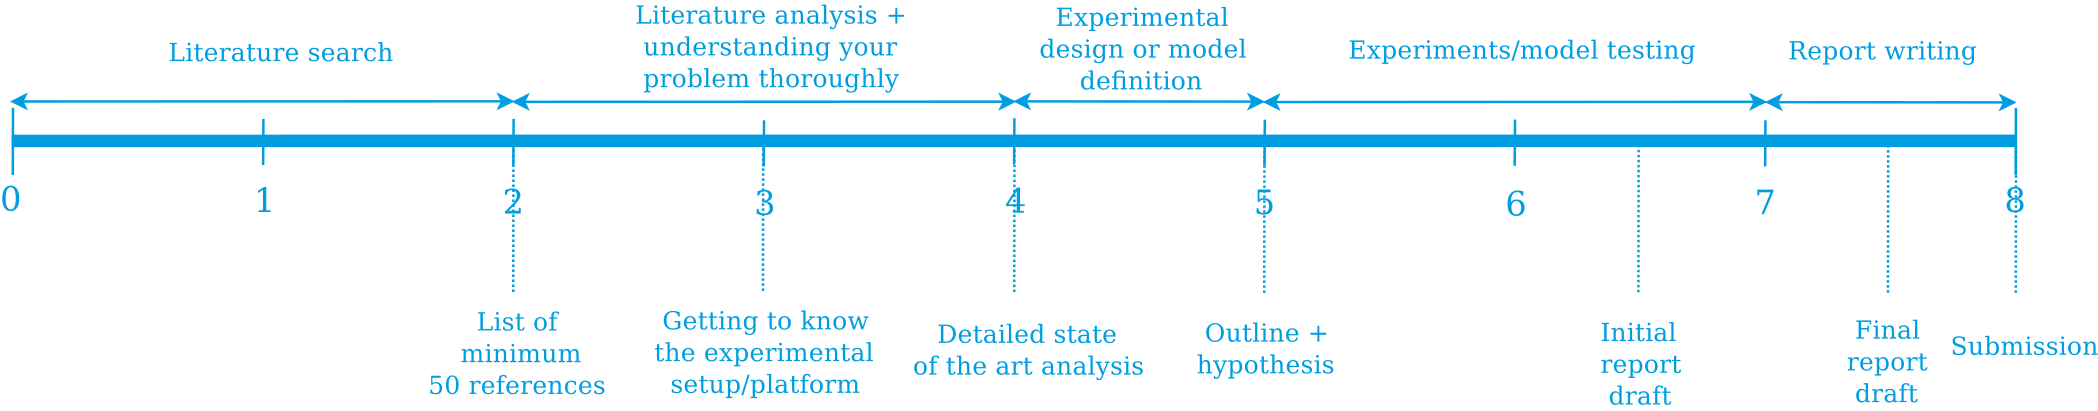
\includegraphics[width=\textwidth]{images/rnd_deliverable_timeline}
    \caption{My figure caption}
    \label{fig:myfigure}
\end{figure}

\subsection{Deliverables}

\subsubsection*{Minimum Viable}
\begin{itemize}
    \item Project results required to get a satisfying or sufficient grade.
\end{itemize}

\subsubsection*{Expected}
\begin{itemize}
    \item Project results required to get a good grade.
\end{itemize}

\subsubsection*{Desired}
\begin{itemize}
    \item Project results required to get an excellent grade.
\end{itemize}

Please note that the final grade will not only depend on the results obtained in your work, but also on how you present the results.

\nocite{*}

\bibliographystyle{plainnat} % Use the plainnat bibliography style
\bibliography{bibliography.bib} % Use the bibliography.bib file as the source of references

\end{document}
